\begin{figure}[htbp]
	\centering
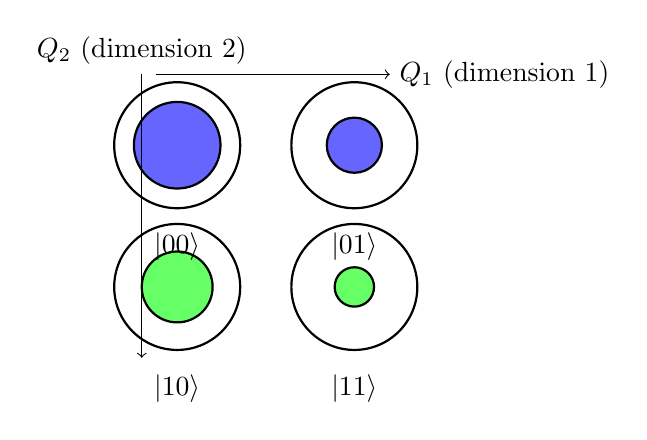
\begin{tikzpicture}[scale=0.9]
	\begin{scope}
		% 2x2 grid: top row |00>, |01>; bottom row |10>, |11>
		\foreach \x/\y/\label in {0/1/00, 2.5/1/01, 0/-1/10, 2.5/-1/11} {
			\node[draw, circle, minimum size=1.6cm, thick] at (\x,\y) {};
		}
		% Inner filled circles
		\foreach \x/\y/\fill/\r in {0/1/blue!60/1.1, 2.5/1/blue!60/0.7, 0/-1/green!60/0.9, 2.5/-1/green!60/0.5} {
			\node[draw, circle, fill=\fill, minimum size=\r cm, thick] at (\x,\y) {};
		}
		% Labels below each circle
		\node[below] at (0,1-1.1) {$|00\rangle$};
		\node[below] at (2.5,1-1.1) {$|01\rangle$};
		\node[below] at (0,-1-1.1) {$|10\rangle$};
		\node[below] at (2.5,-1-1.1) {$|11\rangle$};
	\end{scope}
	
	% Q1 axis (horizontal, left-right) on top of circles
	\draw[->] (-0.3,2.0) -- (3.0,2.0) node[right] {$Q_1$ (dimension 1)};
	% Q2 axis (vertical, top-to-bottom) left of circles
	\draw[->] (-0.5,2.0) -- (-0.5,-2.0) node[pos=0, above] {$Q_2$ (dimension 2)};
	
	\end{tikzpicture}
	\caption{Two-qubit state in Dimensional Circular Notation. Circles are arranged in a $2 \times 2$ grid with explicit dimensional axes $Q_1$ and $Q_2$, corresponding to the two qubits.}
	\label{fig:dcn-2qubit}
\end{figure}
